\documentclass[11pt,a4paper]{article}

% ================= PAQUETES =================
\usepackage[utf8]{inputenc}
\usepackage[T1]{fontenc}
\usepackage[spanish,es-tabla]{babel}
\usepackage[margin=2.5cm]{geometry}
\usepackage{graphicx}
\usepackage{amsmath,amssymb}
\usepackage{xcolor}
\usepackage{hyperref}
\usepackage{booktabs}
\usepackage{caption}
\usepackage{subcaption}
\usepackage[section]{placeins}
\usepackage{tikz}
\usetikzlibrary{arrows.meta,positioning,calc,babel}

\hypersetup{
    colorlinks=true,
    linkcolor=blue,
    citecolor=blue,
    urlcolor=blue,
    pdftitle={TP Final - Robótica Móvil},
}

% ================= CARÁTULA =================
\renewcommand{\topfraction}{0.9}
\renewcommand{\bottomfraction}{0.8}
\renewcommand{\textfraction}{0.07}
\renewcommand{\floatpagefraction}{0.85}
\setcounter{topnumber}{3}
\setcounter{totalnumber}{4}

\setlength{\emergencystretch}{3em}

\begin{document}

\begin{titlepage}
\centering
{
\includegraphics[width=0.2\textwidth]{UBA.png}\par}
\vspace{1cm}
{\bfseries\LARGE Universidad de Buenos Aires \par}
\vspace{0.5cm}
{\scshape\Large Facultad de Ciencias Exactas y Naturales \par}
\vspace{3cm}
{\scshape\Huge Seguimiento de trayectoria a lazo cerrado basado en EKF para un robot omnidireccional \par}
\vspace{1cm}
{\scshape\Large Robótica Móvil -- 2\textsuperscript{do} Cuatrimestre 2025 \par}
\vspace{3cm}
{\itshape\Large Trabajo Práctico Final \par}
\vfill
{\Large
\begin{tabular}{ll}
\textbf{Alumno} & \textbf{L.U.} \\[0.4em]
Iván Agustín Bravo          & 786/23  \\
Pablo Benavente Jacyszyn & 1035/22 \\
\end{tabular}
\par}
\vfill
\end{titlepage}

\tableofcontents
\newpage

% =====================================================================
\section{Introducción}
% Consigna: "Se debe introducir el problema que se está abarcando, dando
% motivaciones y aplicaciones del mismo. Enunciar el enfoque propuesto
% para su resolución."

Los robots móviles omnidireccionales son aquellos que tienen la capacidad de desplazarse en cualquier dirección del plano sin la necesidad de reorientarse previamente. Esto los diferencia de los robots con ruedas convencionales que, al tener sus ruedas alineadas, solo pueden moverse hacia adelante o hacia atrás y deben girar para cambiar de dirección.

En este trabajo se propone lograr que un robot omnidireccional de cuatro ruedas Mecanum pueda seguir una trayectoria de referencia de manera precisa. Para ello, se implementan distintos contenidos desarrollados a lo largo de la cursada de la materia, utilizando el sistema ROS2 y el simulador CoppeliaSim.

El trabajo consta de tres etapas que trabajan en conjunto. La primera consiste en el desarrollo del modelo cinemático del robot, que permite traducir los comandos de velocidad en velocidades de las ruedas Mecanum y, a su vez, estimar la posición del robot a partir de la odometría. En segundo lugar, se implementa un controlador que permite manejar los grados de libertad del robot de forma desacoplada, de manera que pueda realizar el seguimiento de la trayectoria de referencia mediante selección sucesiva de objetivos cercanos. Por último, se incorpora un Filtro de Kalman Extendido (EKF) que permite mejorar la estimación de la posición del robot, utilizando la odometría en conjunto con observaciones de postes del entorno detectados por un sensor láser. Esta estimación mejorada se utiliza como retroalimentación para el controlador, logrando un seguimiento más preciso de la trayectoria deseada.

A lo largo del trabajo se presentan los modelos matemáticos utilizados, las decisiones tomadas durante la implementación y los experimentos realizados junto con sus resultados, a fin de evaluar el desempeño de las estimaciones frente a la pose real del robot.

% =====================================================================
\section{Modelo Cinemático}
\label{sec:modelo}
% Consigna: presentar particularidades de la plataforma, parámetros,
% metodología de odometría, y experimentos que validen el modelo.
\subsection{Plataforma y parámetros}

La plataforma es un robot de cuatro ruedas Mecanum con disposición cuadrada, con una distancia de 350~mm entre ejes. Las ruedas son fijas y cada una cuenta con su propio motor, y tienen la particularidad de tener rodillos a 45° que sirven para transmitir parte de la fuerza de la rueda en dirección de ese ángulo. De esta forma, dependiendo el sentido de giro de cada rueda, las componentes se suman o se cancelan, permitiendo que el robot se desplace en cualquier dirección. 

Cada rueda tiene un encoder absoluto de 500 ticks por revolución, que suma cuando la rueda gira hacia adelante, y resta cuando gira hacia atrás. A su vez, el radio de la rueda es de 50~mm, de manera que cada tick del encoder representa un recorrido de $2\pi r/500 \approx 0.63$ mm, lo que fija el desplazamiento mínimo que la odometría puede detectar. 

Los parámetros del modelo se encuentran resumidos en la siguiente tabla: 

\begin{table}[htbp]
\centering
\begin{tabular}{llc}
\toprule
\textbf{Parámetro} & \textbf{Símbolo} & \textbf{Valor} \\
\midrule
Radio de rueda & $r$ & $0.05$ m \\
Semidistancia entre ruedas & $L = (l_x + l_y)/2$ & $0.175$ m \\
Resolución del encoder & -- & 500 ticks/rev \\
\bottomrule
\end{tabular}
\caption{Parámetros de la plataforma.}
\label{tab:parametros}
\end{table}

\subsection{Cinemática inversa (control de ruedas)}

Se implementó la cinemática inversa propuesta en Taheri et al. \emph{Kinematic Model Of Four Mecanum Wheeled Mobile Robot}~\cite{taheri2015} (ecuación 20) que, dada la velocidad deseada del robot en su propio marco, calcula la velocidad angular que debe tener cada rueda:

\begin{equation}
\begin{bmatrix}\omega_{FL}\\ \omega_{FR}\\ \omega_{RL}\\ \omega_{RR}\end{bmatrix}
= \frac{1}{r}
\begin{bmatrix}
1 & -1 & -(l_x+l_y)\\
1 & 1 & (l_x+l_y)\\
1 & 1 & -(l_x+l_y)\\
1 & -1 & (l_x+l_y)
\end{bmatrix}
\begin{bmatrix}v_x\\ v_y\\ \omega_z\end{bmatrix}
\label{eq:cin_inversa}
\end{equation}

donde $\omega_{FL}$, $\omega_{FR}$, $\omega_{RL}$ y $\omega_{RR}$ son las velocidades angulares de las ruedas del robot, $v_x$ y $v_y$ son las velocidades lineales en los respectivos ejes, $\omega_z$ es la velocidad de giro del robot alrededor de su eje vertical y $r$, $l_x$ y $l_y$ son los parámetros de la plataforma (Tabla~\ref{tab:parametros}). Cada columna de la matriz explica el efecto de cada componente de la velocidad deseada sobre el movimiento de las ruedas. 

El nodo recibe el comando \texttt{geometry\_msgs/Twist} por el tópico \texttt{/robot/cmd\_vel} y publica en los tópicos \texttt{/robot/front\_left\_wheel/cmd\_vel}, \texttt{/robot/front\_right\_wheel/cmd\_vel}, \texttt{/robot/rear\_left\_wheel/cmd\_vel} y \texttt{/robot/rear\_right\_wheel/cmd\_vel} las velocidades de cada rueda (calculadas con la ecuación~\eqref{eq:cin_inversa}).

\subsection{Cinemática directa (odometría)}

Para estimar la pose del robot se implementó el modelo directo propuesto en Taheri et al. \emph{Kinematic Model Of Four Mecanum Wheeled Mobile Robot}~\cite{taheri2015} (ecuaciones 21 a 24) que, con los giros de las ruedas, permite calcular la velocidad del robot. 

El nodo lee los ticks de los encoders de cada rueda por el tópico \texttt{/robot/encoders}. A partir de dos lecturas consecutivas, se utiliza la variación de ticks de cada rueda $i$ para calcular la distancia recorrida: 

\begin{equation}
d_i = \frac{\Delta\text{ticks}_i}{500}\,2\pi r
\end{equation}
y, con estas distancias se calcula el desplazamiento del robot, expresado en su propio marco:
\begin{equation}
\begin{bmatrix}\Delta x_b\\ \Delta y_b\\ \Delta\theta\end{bmatrix}
= \frac{1}{4}
\begin{bmatrix}
1 & 1 & 1 & 1\\
-1 & 1 & 1 & -1\\
-\dfrac{1}{l_x+l_y} & \dfrac{1}{l_x+l_y} & -\dfrac{1}{l_x+l_y} & \dfrac{1}{l_x+l_y}
\end{bmatrix}
\begin{bmatrix}d_1\\ d_2\\ d_3\\ d_4\end{bmatrix}
\label{eq:cin_directa}
\end{equation}

donde los índices 1 a 4 corresponden a las cuatro ruedas del robot (FL, FR, RL, RR). La segunda fila de la matriz permite calcular el desplazamiento lateral del robot, a diferencia de un robot diferencial. 

Para obtener la pose del robot en el marco inercial \texttt{odom}, siendo $(x, y, \theta)$ la pose estimada hasta la lectura anterior, se aplica una rotación según esa orientación $\theta$ a los desplazamientos $\Delta x_b$ y $\Delta y_b$, y se suman a la pose anterior: 

\begin{align}
x &\leftarrow x + \Delta x_b\cos\theta - \Delta y_b\sin\theta\\
y &\leftarrow y + \Delta x_b\sin\theta + \Delta y_b\cos\theta\\
\theta &\leftarrow \theta + \Delta\theta
\end{align}

La pose se inicializa en el origen del marco \texttt{odom}. Al procesar cada lectura de los encoders, el nodo publica la pose estimada y la velocidad del robot como un mensaje \texttt{nav\_msgs/Odometry} en el tópico \texttt{/robot/odometry}, y la pose como la transformación \texttt{odom} $\rightarrow$ \texttt{base\_link} en \texttt{/tf}. En ambos casos, la referencia del tiempo proviene de la lectura de los encoders. 

\subsection{Experimentos}
\label{sec:modelo_exp}
Se realizaron dos tipos de experimentos. El primero compara las velocidades de los comandos contra las velocidades reales del robot. El segundo compara la pose estimada por la odometría contra la pose real del robot. En ambos casos, los valores reales se obtienen de la transformación \texttt{odom} $\rightarrow$ \texttt{base\_link\_gt} publicada por el simulador. 

Para evaluar los distintos movimientos, se realizaron corridas a lazo abierto, en las que se publicó una velocidad constante en \texttt{/robot/cmd\_vel} durante un tiempo fijo. Las corridas se resumen en la Tabla~\ref{tab:corridas_modelo}, y las trayectorias que recorrió el robot en cada una se muestran en la Figura~\ref{fig:modelo_tray}.

\begin{table}[htbp]
\centering
\begin{tabular}{lcccc}
\toprule
\textbf{Corrida} & $v_x$ [m/s] & $v_y$ [m/s] & $\omega_z$ [rad/s] & \textbf{Duración} [s] \\
\midrule
Lateral & $0$ & $-0.3$ & $0$ & $4$ \\
Circular lenta & $0.15$ & $0$ & $-0.3$ & $22$ \\
Circular rápida & $0.3$ & $0$ & $-0.3$ & $23$ \\
Lateral con giro & $0$ & $0.1$ & $0.1$ & $10$ \\
Combinada & $0.1$ & $0.1$ & $0.1$ & $10$ \\
\bottomrule
\end{tabular}
\caption{Consignas de velocidad de las corridas a lazo abierto.}
\label{tab:corridas_modelo}
\end{table}

La corrida lateral evalúa el desplazamiento en $y$, propio del robot omnidireccional.

En las corridas circulares se comandan a la vez una velocidad de avance $v_x$ y una de giro $\omega_z$, ambas constantes, de manera que el robot debería describir una circunferencia de radio $R = v_x/|\omega_z|$, en sentido horario porque $\omega_z$ es negativa. Las dos corridas tienen la misma velocidad de giro, pero en la rápida la velocidad de avance es el doble, lo que lleva el radio de $0.5$~m a $1$~m. Como una vuelta completa demora $2\pi/|\omega_z| \approx 20.9$~s, en ambas el robot recorre algo más de una vuelta. De esta forma, se puede ver el efecto que tiene la velocidad de avance sobre el error, manteniendo el mismo giro.

Las dos últimas corridas combinan desplazamiento lateral con giro, y en la combinada se comandan las tres velocidades a la vez. 

\subsubsection{Velocidades comandadas y reales}

Para comparar las velocidades, se calculó la velocidad real a partir de la pose que informa el simulador, y se la graficó junto con la comandada y con la estimada por la odometría (Figura~\ref{fig:modelo_vel}). En la Tabla~\ref{tab:vel_modelo} se resumen los promedios de cada corrida, sin tener en cuenta el primer segundo ni los últimos $0.2$~s, que corresponden al arranque y al frenado del robot.

\begin{figure}[!htbp]
\centering
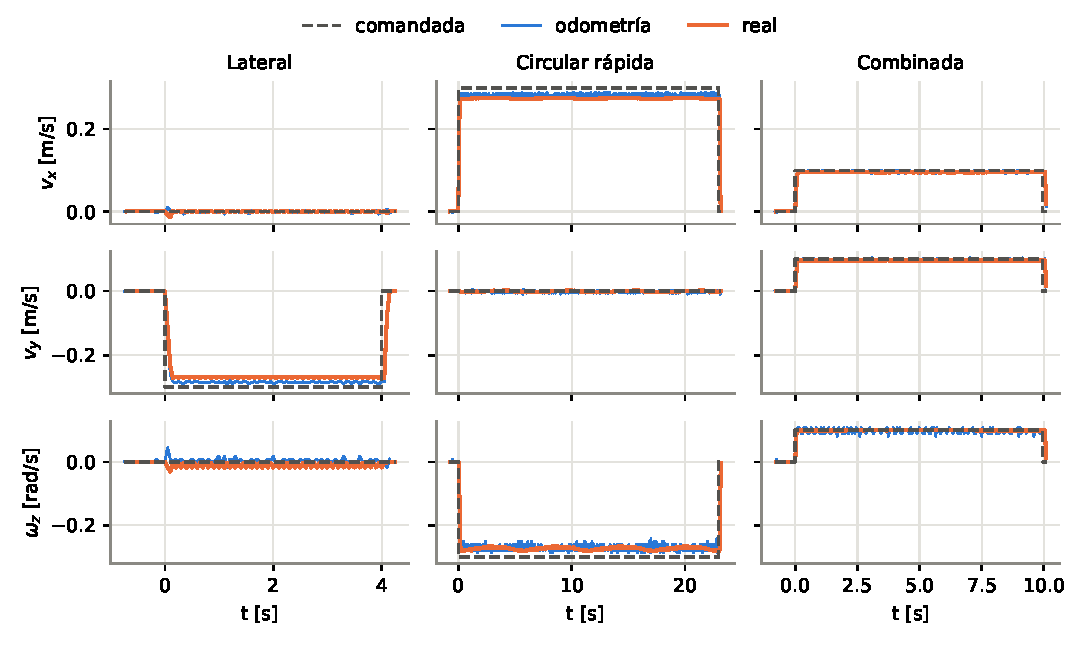
\includegraphics[width=\textwidth]{figuras/modelo_velocidades.pdf}
\caption{Velocidades comandadas, estimadas por la odometría y reales. El comando se empieza a publicar en $t = 0$.}
\label{fig:modelo_vel}
\end{figure}

\begin{table}[!htbp]
\centering
\begin{tabular}{llccc}
\toprule
\textbf{Corrida} & \textbf{Componente} & \textbf{Comandada} & \textbf{Odometría} & \textbf{Real} \\
\midrule
Lateral & $v_y$ [m/s] & $-0.300$ & $-0.285$ & $-0.269$ \\
Circular lenta & $v_x$ [m/s] & $0.150$ & $0.146$ & $0.144$ \\
 & $\omega_z$ [rad/s] & $-0.300$ & $-0.289$ & $-0.289$ \\
Circular rápida & $v_x$ [m/s] & $0.300$ & $0.283$ & $0.275$ \\
 & $\omega_z$ [rad/s] & $-0.300$ & $-0.270$ & $-0.273$ \\
Lateral con giro & $v_y$ [m/s] & $0.100$ & $0.099$ & $0.098$ \\
 & $\omega_z$ [rad/s] & $0.100$ & $0.098$ & $0.100$ \\
Combinada & $v_x$ [m/s] & $0.100$ & $0.097$ & $0.095$ \\
 & $v_y$ [m/s] & $0.100$ & $0.097$ & $0.095$ \\
 & $\omega_z$ [rad/s] & $0.100$ & $0.097$ & $0.100$ \\
\bottomrule
\end{tabular}
\caption{Promedios de las velocidades comandadas, estimadas por la odometría y reales.}
\label{tab:vel_modelo}
\end{table}

En todas las corridas el robot se mueve en la dirección comandada, pero las velocidades lineales reales son algo menores que las comandadas, y la diferencia crece con la velocidad, desde $0.005$~m/s cuando se comandan $0.1$~m/s hasta $0.031$~m/s cuando se comandan $0.3$~m/s. Parte de esta diferencia se debe a que las ruedas no alcanzan la velocidad comandada, y el resto a que el robot se desplaza menos de lo que giran sus ruedas, por el deslizamiento que la odometría no puede detectar.

Las oscilaciones de la velocidad estimada se deben a la resolución de los encoders, ya que un solo tick de diferencia en una rueda cambia la velocidad estimada en unos $0.003$~m/s.

\subsubsection{Pose estimada por odometría y pose real}

Para evaluar la odometría, se comparó la trayectoria en el plano y la orientación estimadas contra las reales. El error de posición y el de orientación se calcularon como
\begin{align}
e_p &= \sqrt{(x_{odom} - x_{gt})^2 + (y_{odom} - y_{gt})^2}\\
e_\theta &= \theta_{odom} - \theta_{gt}
\end{align}
donde el subíndice $gt$ indica los valores reales informados por el simulador y $e_\theta$ se normaliza al intervalo $(-\pi, \pi]$.

Las trayectorias y las orientaciones de cada corrida, expresadas en el marco \texttt{odom}, se presentan en las Figuras~\ref{fig:modelo_tray} y~\ref{fig:modelo_ori}, y los errores se resumen en la Tabla~\ref{tab:error_odom}.




\begin{figure}[!htbp]
\centering
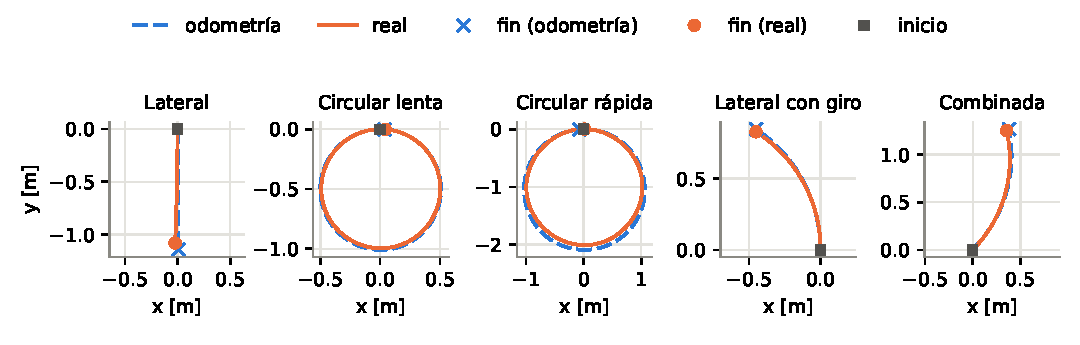
\includegraphics[width=\textwidth]{figuras/modelo_trayectorias.pdf}
\caption{Trayectorias estimadas por la odometría y reales.}
\label{fig:modelo_tray}
\end{figure}

En todas las corridas, la trayectoria estimada tiene la misma forma que la real. En la lateral, la mayor parte del error está en la dirección del movimiento, ya que la odometría estima un desplazamiento de $1.15$~m mientras que el robot se desplaza $1.08$~m. A su vez, el robot termina girado $2.4^\circ$ en sentido horario, pero la odometría estima un giro de $0.9^\circ$ en sentido antihorario.

\begin{table}[!htbp]
\centering
\begin{tabular}{lcccc}
\toprule
\textbf{Corrida} & \textbf{Recorrido real} [m] & $e_p$ \textbf{final} [cm] & $e_p$ \textbf{máximo} [cm] & $e_\theta$ \textbf{final} \\
\midrule
Lateral & $1.08$ & $7.2$ & $7.3$ & $3.3^\circ$ \\
Circular lenta & $3.18$ & $0.5$ & $1.5$ & $0.1^\circ$ \\
Circular rápida & $6.32$ & $8.3$ & $11.6$ & $4.4^\circ$ \\
Lateral con giro & $0.98$ & $1.9$ & $1.9$ & $-1.4^\circ$ \\
Combinada & $1.35$ & $3.0$ & $3.1$ & $-1.6^\circ$ \\
\bottomrule
\end{tabular}
\caption{Errores de la odometría respecto de la pose real.}
\label{tab:error_odom}
\end{table}

\begin{figure}[!htbp]
\centering
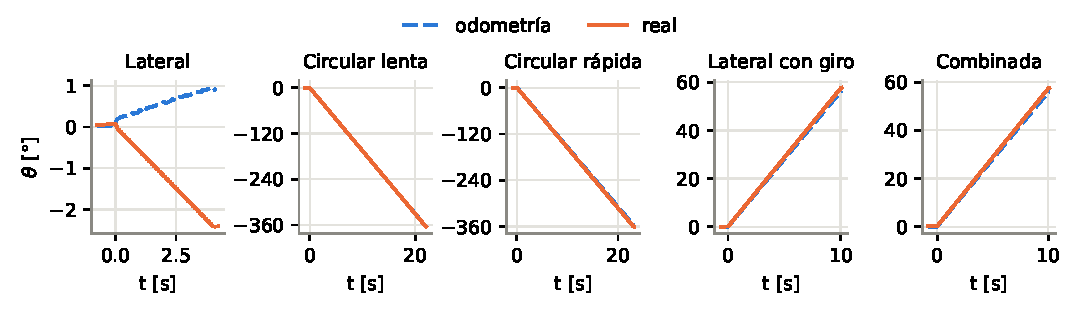
\includegraphics[width=\textwidth]{figuras/modelo_orientacion.pdf}
\caption{Orientaciones estimadas por la odometría y reales. La escala vertical es distinta en cada corrida.}
\label{fig:modelo_ori}
\end{figure}

En las circulares se puede ver el efecto de la velocidad de avance, dado que al duplicarla el recorrido también se duplica, pero el error máximo aumenta mucho más, de $1.5$~cm a $11.6$~cm. El error final es menor que el máximo porque el robot vuelve cerca del punto de partida, de manera que parte del error acumulado se compensa.

\subsubsection{Análisis del error}

Para identificar el origen del error, se comparó la velocidad estimada por la odometría con la real (Tabla~\ref{tab:vel_modelo}). Si el error se debiera a un parámetro del modelo, como el radio de las ruedas, ambas velocidades diferirían siempre en la misma proporción. Sin embargo, la diferencia aumenta con la velocidad y es mayor en el desplazamiento lateral, lo que indica que el robot se desplaza menos de lo que giran sus ruedas, es decir, que las ruedas deslizan. A su vez, esto coincide con los errores de pose de la Tabla~\ref{tab:error_odom}, de manera que las corridas en las que más deslizan las ruedas, la lateral y la circular rápida, son también las que terminan con mayor error. Como los encoders solo miden el giro de cada rueda, la odometría no puede detectar este error, que se acumula a medida que el robot avanza, y por eso se lo corrige con las observaciones de los postes en el EKF de la Sección~\ref{sec:ekf}.

% =====================================================================
\section{Control a lazo cerrado y seguimiento de trayectorias}
\label{sec:lazo_cerrado}
\subsection{Controlador Proporcional}

Los tres grados de libertad ($x$, $y$ y $\theta$), pueden controlarse de manera independiente dado que se trata de un robot holonómico. Se implementó un controlador proporcional (P) para cada uno de estos grados. En cada iteración se compara la pose actual del robot $(x, y, \theta)$ con la pose objetivo $(x_g, y_g, \theta_g)$ y se calcula el error en el marco inercial:

\begin{equation}
e_{x,w} = x_g - x, \qquad e_{y,w} = y_g - y, \qquad e_\theta = \mathrm{norm}(\theta_g - \theta)
\end{equation}
donde $\mathrm{norm}(\cdot)$ lleva el ángulo al intervalo $(-\pi, \pi]$, para que el robot siempre gire por el camino más corto. Como el comando de velocidad se expresa en el marco del robot, el error de posición se rota según la orientación actual:
\begin{equation}
\begin{bmatrix} e_{x,b} \\ e_{y,b} \end{bmatrix} =
\begin{bmatrix} \cos\theta & \sin\theta \\ -\sin\theta & \cos\theta \end{bmatrix}
\begin{bmatrix} e_{x,w} \\ e_{y,w} \end{bmatrix}
\end{equation}
y la ley de control es:
\begin{equation}
v_x = k_{p,xy}\, e_{x,b}, \qquad v_y = k_{p,xy}\, e_{y,b}, \qquad \omega_z = k_{p,yaw}\, e_\theta
\label{eq:ley_control}
\end{equation}

Las velocidades resultantes se publican en \texttt{/robot/cmd\_vel} como un \texttt{Twist}, que el modelo cinemático convierte en velocidades de rueda. La pose actual se obtiene de la transformación \texttt{map} $\rightarrow$ \texttt{base\_link}, que cierra el lazo (Figura~\ref{fig:lazo_cerrado}).

\begin{figure}[htbp]
\centering
\begin{tikzpicture}[scale=0.8, transform shape, node distance=2.2cm, >=Stealth,
  blk/.style={draw, rectangle, minimum width=2.4cm, minimum height=1cm, align=center}]
  \node (sp) {$(x_g,y_g,\theta_g)$};
  \node[circle, draw, right=1.2cm of sp] (sum) {};
  \node[blk, right=1.2cm of sum] (rot) {Rotación\\a marco robot};
  \node[blk, right=1.2cm of rot] (p) {Controlador P};
  \node[blk, right=2.6cm of p] (rob) {Robot};
  \node[right=1.2cm of rob] (out) {$(x,y,\theta)$};
  \node[blk, below=1.2cm of p] (odo) {Odometría};
  \draw[->] (sp) -- (sum);
  \draw[->] (sum) -- node[above] {$e$} (rot);
  \draw[->] (rot) -- node[above] {$e_b$} (p);
  \draw[->] (p) -- node[above, font=\small] {$v_x,v_y,\omega_z$} (rob);
  \draw[->] (rob) -- (out);
  \draw[->] ($(rob.east)+(0.6,0)$) |- (odo.east);
  \draw[->] (odo.west) -| node[pos=0.95, left] {$-$} (sum.south);
\end{tikzpicture}
\caption{Lazo cerrado del controlador de pose.}
\label{fig:lazo_cerrado}
\end{figure}

\subsection{Trayectoria cuadrada y \emph{pursuit-based following}}
\label{sec:trayectoria}

La trayectoria de referencia es un cuadrado centrado en el origen del mapa.{\renewcommand{\thefootnote}{\fnsymbol{footnote}}\footnote{El enunciado indica un cuadrado de 2~m de lado, pero en la figura de la consigna los vértices están en $(\pm 2, \pm 2)$, lo que corresponde a 4~m de lado. Para la implementación se tomaron los vértices de la figura.}} El robot debe recorrerla en sentido antihorario, manteniendo una orientación opuesta al centro. Para definir esta orientación se siguió la figura de la consigna, en la que el robot está orientado a $90^\circ$ en el vértice $(-2, 2)$, a $180^\circ$ en $(-2, -2)$, a $270^\circ$ en $(2, -2)$ y a $360^\circ$ en $(2, 2)$, es decir, gira $90^\circ$ en sentido antihorario en cada lado. Notar que en las figuras de este informe el eje $x$ del marco \texttt{map} se dibuja hacia la derecha y el eje $y$ hacia arriba, de manera que el cuadrado se ve girado $90^\circ$ respecto de la figura de la consigna.

Entre dos vértices, la orientación objetivo se interpola linealmente
\begin{equation}
\theta_g = \theta_i + \frac{\pi}{2}\,u
\end{equation}
donde $\theta_i$ es la orientación en el vértice en el que comienza el lado y $u \in [0, 1]$ es la fracción del lado recorrida. El recorrido comienza en $(-2, 2)$, donde la orientación objetivo coincide con la orientación inicial del robot en el simulador.

Esta orientación puede mantenerse a lo largo de todo el recorrido porque el robot es holonómico, de manera que puede seguir la trayectoria sin girar hacia la dirección del movimiento.

Para que el controlador pueda seguir la trayectoria, el nodo \texttt{trajectory\_generator} la divide en una lista de waypoints discretos, separados 0.05~m, cada uno con una posición y una orientación $\theta_g$, y la publica en \texttt{/robot/trajectory}. 

El controlador lleva al robot hacia una pose objetivo. Si esa pose fuera el último punto de la trayectoria, el robot iría directo hacia él en lugar de seguir el cuadrado. Por eso el objetivo se actualiza a medida que el robot avanza, eligiendo siempre un waypoint cercano de la lista (\emph{pursuit-based goal selection}). El objetivo se elige de la siguiente manera:

\begin{itemize}
    \item Al comenzar, se toma como punto de partida el waypoint más cercano al robot.
    \item En cada iteración, se recorre la lista desde el último objetivo y se elige el primer waypoint que está a más de una distancia de anticipación (\emph{lookahead}) del robot. Su valor se elige en la Sección~\ref{sec:lazo_exp}.
    \item Cuando ya no quedan waypoints más allá del \emph{lookahead}, el objetivo es el último punto de la trayectoria. La trayectoria se da por terminada cuando el robot está a menos de $0.05$~m de ese punto y su orientación difiere en menos de $0.05$~rad.
\end{itemize}

De esta forma, el robot persigue un punto que siempre se encuentra por delante, a una distancia aproximadamente igual al \emph{lookahead}. 


\subsection{Experimentos}
\label{sec:lazo_exp}
Para elegir las constantes del controlador, se realizaron corridas en las que el robot sigue la trayectoria cuadrada completa, utilizando la odometría como retroalimentación y un \emph{lookahead} de $0.30$~m. Se probaron tres valores de $k_{p,xy}$ y tres de $k_{p,yaw}$, variando una constante a la vez y dejando la otra fija, y de cada configuración se realizó una sola corrida.

En la Tabla~\ref{tab:barrido} se resumen los resultados. Las columnas $d$, $e_p$ y $e_\theta$ corresponden al robot real, siendo $d$ su distancia al cuadrado a lo largo del recorrido, y $e_p$ y $e_\theta$ los errores de posición y de orientación con los que termina respecto del punto de llegada. Las dos últimas columnas corresponden a la pose estimada por la odometría, que es la que ve el controlador, siendo $\bar{e}_{p,tray}$ la distancia media de esa pose al cuadrado, y $\bar{e}_{\theta,tray}$ el error medio entre su orientación y la que corresponde al lugar de la trayectoria en el que se encuentra el robot. La duración se mide en tiempo de simulación, desde el primer comando hasta que el controlador da por terminada la trayectoria.

\begin{table}[htbp]
\centering
\small
\setlength{\tabcolsep}{4pt}
\begin{tabular}{ccccccccc}
\toprule
$k_{p,xy}$ & $k_{p,yaw}$ & Duración [s] & $d$ medio [m] & $d$ máx. [m] & $e_p$ final [m] & $e_\theta$ final & $\bar{e}_{p,tray}$ [cm] & $\bar{e}_{\theta,tray}$ \\
\midrule
$0.4$ & $1.5$ & $123$ & $0.20$ & $0.54$ & $0.90$ & $19.9^\circ$ & $1.3$ & $5.3^\circ$ \\
$0.8$ & $1.5$ & $64$ & $0.22$ & $0.56$ & $0.90$ & $20.8^\circ$ & $1.5$ & $3.4^\circ$ \\
$1.6$ & $1.5$ & $38$ & $0.42$ & $1.13$ & $2.12$ & $49.4^\circ$ & $2.3$ & $1.4^\circ$ \\
\midrule
$0.8$ & $0.75$ & $65$ & $0.22$ & $0.55$ & $0.88$ & $19.5^\circ$ & $1.5$ & $0.7^\circ$ \\
$0.8$ & $3.0$ & $65$ & $0.23$ & $0.59$ & $1.00$ & $22.9^\circ$ & $1.4$ & $5.3^\circ$ \\
\bottomrule
\end{tabular}
\caption{Resultados de las corridas con distintas constantes.}
\label{tab:barrido}
\end{table}

En todas las corridas la trayectoria estimada sigue al cuadrado, con una distancia media de entre $1.3$ y $2.3$~cm, y el controlador da por terminado el recorrido, pero el robot real se va desviando y termina lejos del punto de llegada (Figura~\ref{fig:lazo_tray}). Esto se debe a que el controlador corrige el error respecto de la pose estimada, de manera que no puede detectar el error propio de la odometría que se vio en la Sección~\ref{sec:modelo_exp}. A su vez, la trayectoria estimada recorta las esquinas hasta $0.14$~m, dado que el objetivo pasa al lado siguiente antes de que el robot llegue al vértice.

\begin{figure}[htbp]
\centering
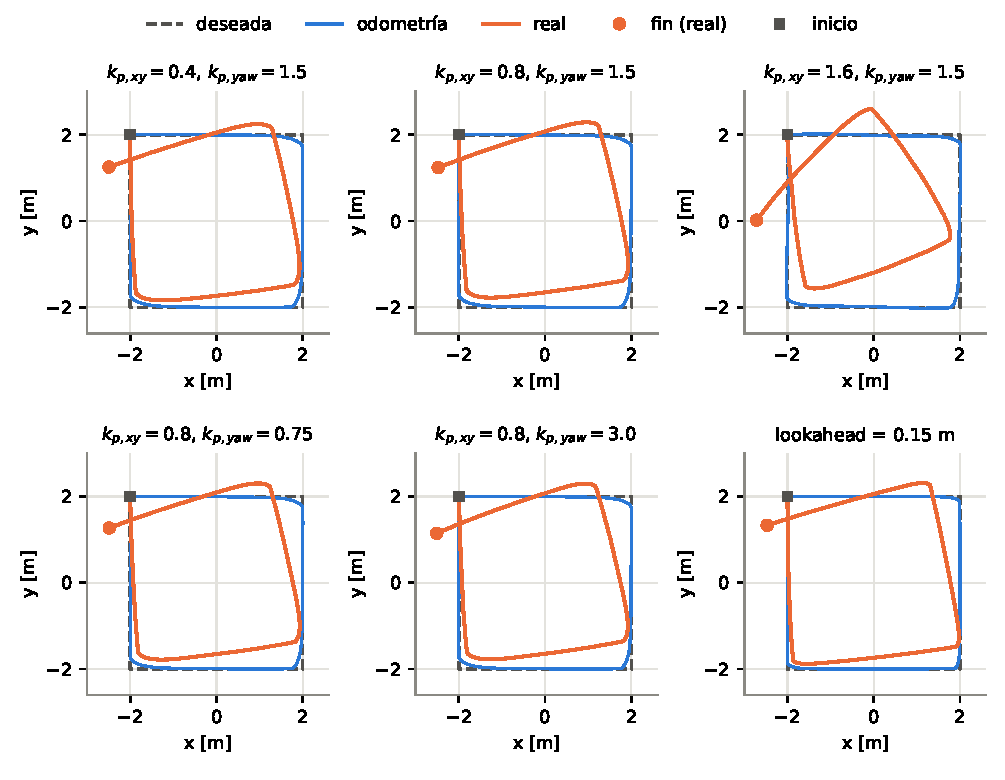
\includegraphics[width=\textwidth]{figuras/lazo_trayectorias.pdf}
\caption{Trayectoria deseada, estimada por la odometría y real.}
\label{fig:lazo_tray}
\end{figure}

\subsubsection{Variación de $k_{p,xy}$}

La pose objetivo, la estimada y la real para los tres valores de $k_{p,xy}$ se presentan en la Figura~\ref{fig:lazo_kpxy}.

\begin{figure}[htbp]
\centering
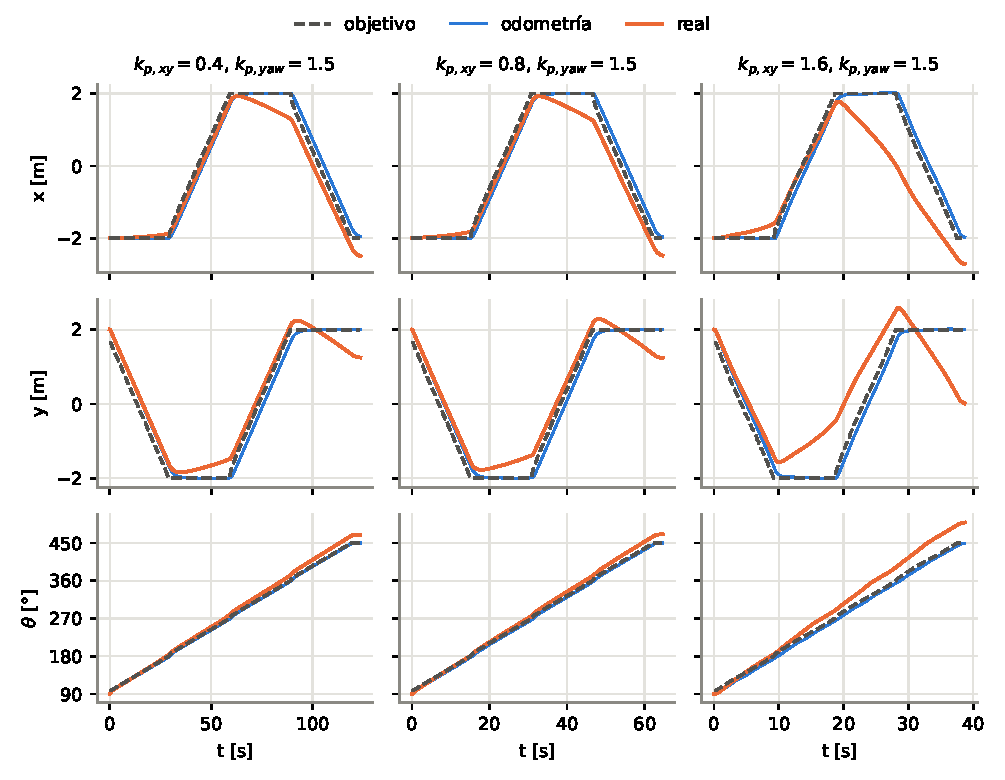
\includegraphics[width=\textwidth]{figuras/lazo_kpxy.pdf}
\caption{Pose objetivo, estimada por la odometría y real para distintos valores de $k_{p,xy}$.}
\label{fig:lazo_kpxy}
\end{figure}

El objetivo siempre está a una distancia aproximadamente igual al \emph{lookahead}, de manera que el error de posición que ve el controlador es casi constante y $k_{p,xy}$ es la que determina la velocidad. Al duplicar la constante se duplica la velocidad del robot, y el recorrido se completa en casi la mitad del tiempo. Con $k_{p,xy} = 0.4$ la velocidad comandada promedio es de $0.13$~m/s, y pasa a $0.26$~m/s con $0.8$ y a $0.51$~m/s con $1.6$. El error del robot real es similar con los dos primeros valores, pero con $1.6$ el error final pasa a ser más del doble, tanto en posición como en orientación. Esto coincide con lo que se vio en la Sección~\ref{sec:modelo_exp}, en la que el error de la odometría es mayor a velocidades más altas.

\subsubsection{Variación de $k_{p,yaw}$}

Para los tres valores de $k_{p,yaw}$, los resultados se presentan en la Figura~\ref{fig:lazo_kpyaw}.

\begin{figure}[htbp]
\centering
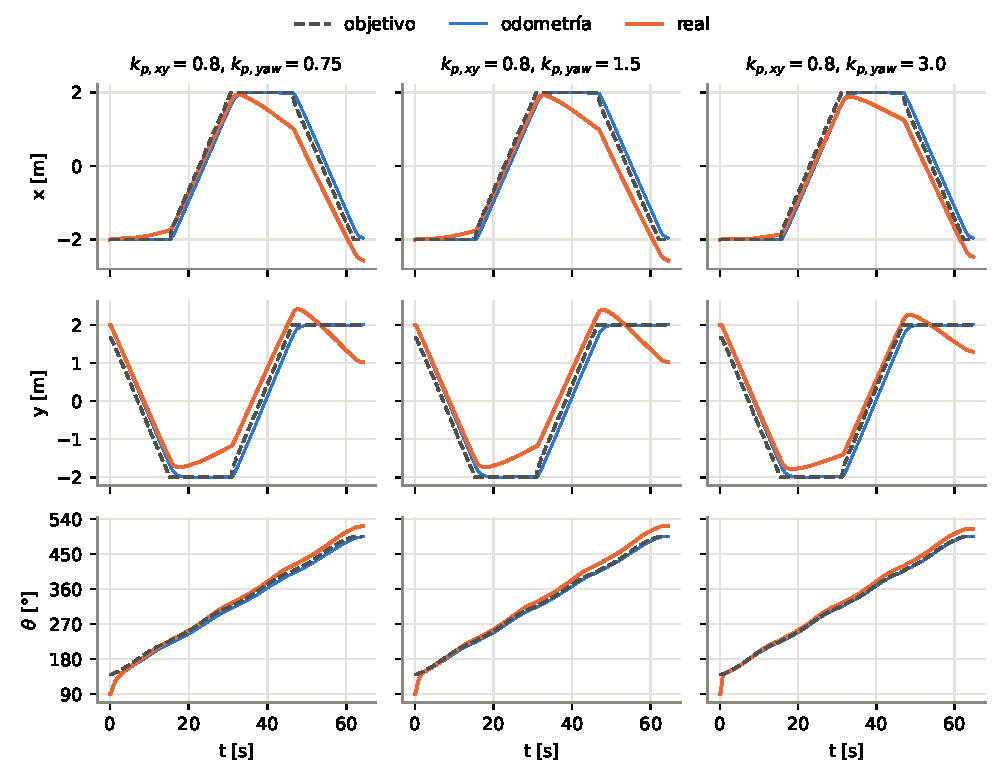
\includegraphics[width=\textwidth]{figuras/lazo_kpyaw.pdf}
\caption{Pose objetivo, estimada por la odometría y real para distintos valores de $k_{p,yaw}$.}
\label{fig:lazo_kpyaw}
\end{figure}

La orientación objetivo cambia a lo largo de todo el recorrido, de manera que el robot siempre la sigue con un retraso. Según la ley de control~\eqref{eq:ley_control}, para que el robot gire a una velocidad $\omega_z$ tiene que haber un error $e_\theta = \omega_z / k_{p,yaw}$, es decir, el retraso se reduce a la mitad al duplicar la constante. La velocidad angular promedio de estas corridas es de $0.105$~rad/s, por lo que el error debería ser de unos $8.0^\circ$ con $k_{p,yaw} = 0.75$, $4.0^\circ$ con $1.5$ y $2.0^\circ$ con $3.0$, y los valores obtenidos fueron de $7.7^\circ$, $3.8^\circ$ y $1.8^\circ$. La duración no cambia, ya que depende de la velocidad lineal.

Sin embargo, el controlador no utiliza la orientación del lugar en el que se encuentra el robot, sino la del objetivo, que está $0.30$~m más adelante. Como en cada lado de $4$~m la orientación gira $90^\circ$, en esos $0.30$~m ya giró unos $6.75^\circ$, de manera que si el robot alcanzara la orientación objetivo, quedaría girado de más para su posición. Con $k_{p,yaw} = 0.75$, el retraso de $7.7^\circ$ casi compensa este adelanto, y el robot queda orientado según la trayectoria con un error de $0.7^\circ$. Con las otras dos constantes, en cambio, el retraso es menor, y el robot queda girado de más, con un error de $3.4^\circ$ y $5.3^\circ$.

En el robot real, el error es prácticamente el mismo con $0.75$ y con $1.5$, y con $3.0$ es algo mayor, dado que el error final de posición llega a $1.00$~m y el de orientación a $22.9^\circ$.

\subsubsection{Velocidades asignadas}

Las velocidades que asignó el controlador en cada momento se presentan en la Figura~\ref{fig:lazo_vel}.

\begin{figure}[htbp]
\centering
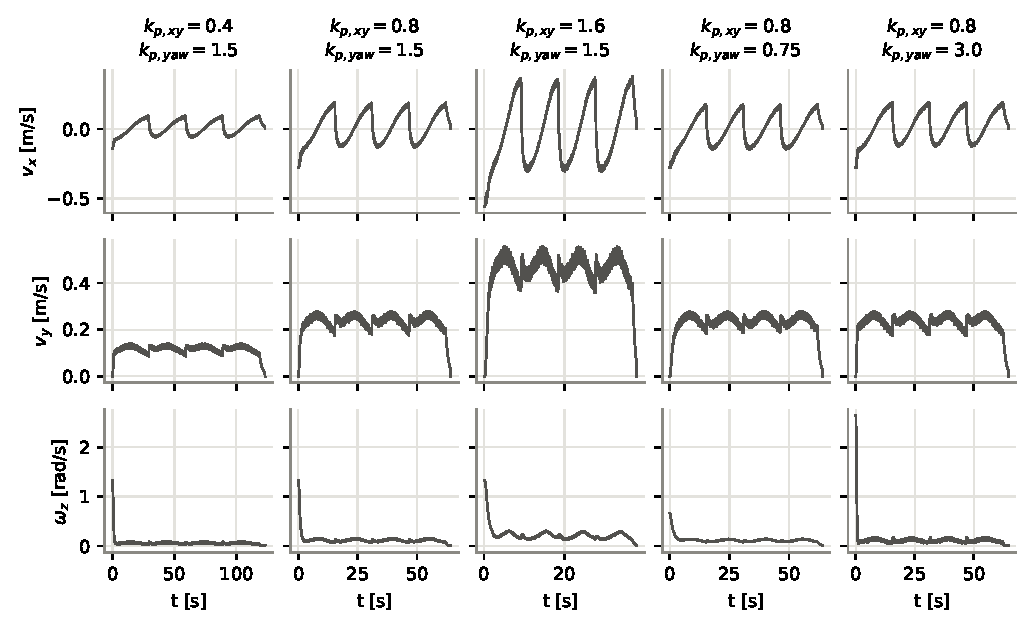
\includegraphics[width=\textwidth]{figuras/lazo_velocidades.pdf}
\caption{Velocidades asignadas por el controlador para distintos valores de las constantes.}
\label{fig:lazo_vel}
\end{figure}

Al comenzar cada lado del cuadrado, el robot está de espaldas a la dirección en la que se mueve, de manera que $v_x$ es negativa y $v_y$ es chica. A medida que avanza va girando, y al final del lado se mueve de costado, con $v_x$ cercana a cero y $v_y$ máxima. Los cambios bruscos corresponden a los vértices, en los que cambia la dirección del movimiento. A su vez, como la orientación objetivo varía linealmente, $\omega_z$ se mantiene casi constante a lo largo de cada lado, salvo por los picos que aparecen al comenzar y en los vértices, que son mayores cuanto mayor es $k_{p,yaw}$. Los de los vértices se deben a que, al pasar al lado siguiente, el objetivo avanza sobre la trayectoria más rápido que el robot.

Además, las velocidades presentan una oscilación rápida, que se debe a que el objetivo avanza de a un waypoint. Cada vez que lo hace, la distancia al objetivo cambia en $0.05$~m, lo que con $k_{p,xy} = 0.8$ modifica la velocidad lineal en $0.04$~m/s.

\subsubsection{Elección de las constantes}

Se eligieron $k_{p,xy} = 0.8$ y $k_{p,yaw} = 0.75$, con un \emph{lookahead} de $0.30$~m. Con estas constantes el robot real obtuvo el menor error final de posición, si bien las diferencias con las demás corridas a la misma velocidad son chicas y solo se realizó una corrida de cada configuración. Lo que define la elección es que, como se vio, con $k_{p,yaw} = 0.75$ el robot se mantiene orientado según el punto de la trayectoria en el que se encuentra, con un error medio de $0.7^\circ$. Por el otro lado, se mantuvo $k_{p,xy} = 0.8$, dado que con $0.4$ el recorrido tarda casi el doble sin que el error mejore, y con $1.6$ el error final se duplica.

El error que queda no puede corregirse ajustando las constantes, ya que el controlador sigue correctamente a la pose estimada y es esta última la que se aparta de la real. Para reducirlo es necesario mejorar la estimación de la pose, para lo que se utiliza el EKF de la Sección~\ref{sec:ekf}.

% =====================================================================
\section{Localización basada en EKF}
\label{sec:ekf}
\subsection{Detección de landmarks (postes)}
\label{sec:landmarks}

Para corregir la estimación de la pose del robot, se utilizan los postes del mapa como referencias (\emph{landmarks}). El nodo \texttt{landmark\_detector} recibe las lecturas del láser por \texttt{/robot/front\_laser/scan} y detecta los postes mediante clusterización de la siguiente manera:

\begin{enumerate}
    \item \textbf{Conversión a cartesianas.} Cada medición válida del escaneo, de rango $r_i$ y ángulo $\alpha_i$, se convierte al punto $(r_i\cos\alpha_i,\ r_i\sin\alpha_i)$ en el marco del láser, y luego se lleva al marco del robot (\texttt{base\_link}) con la transformación \texttt{base\_link} $\rightarrow$ \texttt{front\_laser}. Se descartan las mediciones no finitas o fuera del rango permitido (hasta 8~m).
    \item \textbf{Clusterización secuencial.} Los puntos se recorren en el orden del escaneo y se agrupan: un punto pertenece al mismo grupo que el anterior si la distancia entre ambos es menor a $0.15$~m. Cuando la distancia lo supera, el grupo actual se cierra y se abre uno nuevo.
    \item \textbf{Filtrado.} Un grupo se acepta como poste solo si tiene entre 2 y 30 puntos. Esto descarta mediciones aisladas y objetos más grandes que un poste.
\end{enumerate}

De cada grupo, se promedian los puntos para calcular el centroide, y se lo expresa como un rango y un ángulo con respecto al robot:

\begin{equation}
r = \sqrt{c_x^2 + c_y^2}, \qquad \varphi = \mathrm{atan2}(c_y, c_x)
\end{equation}

Sin embargo, el láser solo alcanza la cara del poste que queda frente al robot, por lo que los puntos de cada grupo están sobre esa cara y su centroide no coincide con el centro del poste, sino que queda más cerca del robot. Si los rayos caen de manera aproximadamente uniforme a lo ancho del poste, la distancia media de los puntos al plano que pasa por el centro es $\pi r_p/4$, siendo $r_p$ el radio del poste, de manera que el centroide queda a esa distancia del centro, que para los postes de $5$~cm de radio es de unos $3.9$~cm. Por eso, antes de calcular $r$ y $\varphi$, el centroide se corre esa distancia en la dirección que va del láser al poste. Comparando las observaciones con las que se obtendrían desde la pose real, el error medio del rango pasó de $-3.9$~cm a menos de $1$~mm con esta corrección.

Las observaciones de los landmarks se publican en \texttt{/landmarks} como un mensaje \texttt{LandmarkArray} del paquete \texttt{robmovil\_msgs}, en el marco del robot y con la marca del escaneo del cual provienen. Además, en \texttt{/landmark\_markers} se publican marcadores de cada poste para poder visualizarlos en RViz2.

\subsection{Modelo del EKF}
\label{sec:modelo_ekf}

El filtro combina la odometría, que predice el movimiento del robot, y las observaciones de los postes, que permiten corregir esa estimación. En esta sección definimos lo que estima el filtro y los modelos que necesita para hacerlo. 

\paragraph{Estado.} El filtro estima la pose del robot en el marco \texttt{map}:
\begin{equation}
\vec{x} = [p_x,\ p_y,\ \theta]^T
\end{equation} 
siendo $(p_x, p_y)$ la posición y $\theta$ la orientación.

\paragraph{Predicción.} La odometría informa la velocidad del robot, medida en su propio marco ($v_x$ hacia adelante, $v_y$ hacia el costado y $\omega$ de giro). Los tres valores son la entrada de control del filtro, $\vec{u} = [v_x,\ v_y,\ \omega]^T$, y se toman del mensaje de \texttt{/robot/odometry}. 

Para actualizar la pose, se multiplica la velocidad por el tiempo $\Delta t$ entre dos mensajes de odometría, se rota el desplazamiento con el ángulo $\theta$ y se suma a la pose anterior, de modo que quede expresada en el marco \texttt{map}:

\begin{equation}
f(\vec{x},\vec{u},\vec{w}) =
\begin{bmatrix}
p_x + (v_x\cos\theta - v_y\sin\theta)\,\Delta t + w_x \\
p_y + (v_x\sin\theta + v_y\cos\theta)\,\Delta t + w_y \\
\theta + \omega\,\Delta t + w_\theta
\end{bmatrix}
\end{equation}

Como la odometría no es perfecta, se suma un ruido $\vec{w} = [w_x,\ w_y,\ w_\theta]^T$ gaussiano, de media 0 y covarianza $Q$.

\paragraph{Corrección.} Como cada poste se encuentra en una posición conocida del mapa $(m_x, m_y)$, si el robot estuviera en la pose $\vec{x}$, debería medir el poste a una distancia $r$ y con un ángulo $\varphi$ respecto de su frente.

\begin{equation}
h(\vec{x},\vec{v}) =
\begin{bmatrix}
\sqrt{(m_x - p_x)^2 + (m_y - p_y)^2} + v_r \\
\mathrm{atan2}(m_y - p_y,\ m_x - p_x) - \theta + v_\varphi
\end{bmatrix}
\end{equation}

La medición esperada se compara con la medición del detector, $\vec{z} = [r,\ \varphi]^T$ (Sección~\ref{sec:landmarks}). La diferencia entre ambas se utiliza para corregir la pose. Notar que, como la medición real también tiene error, se le suma un ruido $\vec{v} = [v_r,\ v_\varphi]^T$ gaussiano, de media 0 y covarianza $R$.

\paragraph{Linealización.} Como $f$ y $h$ no son lineales, el EKF las aproxima con los Jacobianos $J_f$ y $J_h$, que son las matrices de derivadas parciales de cada función con respecto a $\vec{x}$. 

\begin{equation}
J_f =
\begin{bmatrix}
1 & 0 & -(v_x\sin\theta + v_y\cos\theta)\,\Delta t \\
0 & 1 & \phantom{-}(v_x\cos\theta - v_y\sin\theta)\,\Delta t \\
0 & 0 & 1
\end{bmatrix}
\end{equation}
y para el de sensado, con $d_x = m_x - p_x$, $d_y = m_y - p_y$ y $q = d_x^2 + d_y^2$:
\begin{equation}
J_h =
\begin{bmatrix}
-d_x/\sqrt{q} & -d_y/\sqrt{q} & 0 \\
\phantom{-}d_y/q & -d_x/q & -1
\end{bmatrix}
\end{equation}

La componente angular de la diferencia entre la medición y la medición esperada se normaliza siempre al intervalo $(-\pi, \pi]$ para evitar discontinuidades.

El filtro se implementó con la clase \texttt{EKFilter}, que es la que utiliza el paquete \texttt{robmovil\_ekf} de la materia. Como en el robot omnidireccional la entrada $\vec{u}$ tiene tres componentes, las dimensiones se declararon como \texttt{EKFilter(3, 3, 3, 2, 2)}, tal como se indica en el anexo de la consigna. La clase también requiere los Jacobianos de $f$ con respecto a $\vec{w}$ y de $h$ con respecto a $\vec{v}$, que en este caso son la identidad porque los ruidos se suman directamente a la pose y a la medición.

\subsection{Matrices de covarianza}

El filtro requiere tres matrices de covarianza: $Q$ para el ruido de la predicción, $R$ para el ruido de la medición y $P_0$ para la incertidumbre de la pose inicial. La consigna pide proponer matrices iniciales que reflejen una mayor incertidumbre al predecir la pose que al medir, de manera que la información de los sensores se considere más confiable. Todas las matrices son diagonales porque se asume que los errores de cada componente son independientes entre sí. 

\paragraph{Ruido de proceso.}
\begin{equation}
Q = \mathrm{diag}(\sigma_x^2,\ \sigma_y^2,\ \sigma_\theta^2) = \mathrm{diag}(0.02^2,\ 0.02^2,\ 0.01^2)
\end{equation}
con $\sigma_x$ y $\sigma_y$ en metros y $\sigma_\theta$ en radianes. La matriz $Q$ se suma en cada paso de predicción sin escalarla por $\Delta t$, y como la odometría se publica cada $0.05$~s, equivale a una incertidumbre que crece con el tiempo, aunque el robot esté quieto. Por ejemplo, si durante un segundo el robot no ve ningún poste, se suma $Q$ veinte veces y el desvío en cada coordenada llega a unos $0.02\sqrt{20} \approx 9$~cm. Si bien estos valores son mayores que el error real de la odometría en un paso, que en la corrida con las constantes elegidas fue de unos $0.4$~mm en promedio, de esta forma el filtro considera más confiable la medición, como pide la consigna.

\paragraph{Ruido de medición.}
\begin{equation}
R = \mathrm{diag}(\sigma_r^2,\ \sigma_\varphi^2) = \mathrm{diag}(0.01^2,\ 0.005^2)
\end{equation}
con $\sigma_r$ en metros y $\sigma_\varphi$ en radianes ($0.005$~rad $\approx 0.3^\circ$). Para elegirlos, se comparó cada observación del detector con la que debería haberse medido desde la pose real del robot. El desvío fue de unos $2$ a $3$~mm en el rango y de $0.0014$ a $0.0026$~rad en el ángulo, es decir, el láser del simulador mide con mucha precisión, y los valores de $R$ se tomaron algo mayores para dejar un margen.

\paragraph{Relación entre $Q$ y $R$.}
Si bien $Q$ describe errores en la pose del robot y $R$ errores en la medición, se pueden comparar porque unos se trasladan casi directamente a los otros. Si el robot está desplazado una cierta distancia en la dirección del poste, el rango medido cambia esa misma distancia, ya que la primera fila de $J_h$ es un vector unitario en esa dirección, y si el robot está girado un cierto ángulo, el ángulo medido cambia lo mismo pero con signo opuesto, debido al $-1$ de la segunda fila de $J_h$. Comparando las varianzas, la de la predicción es $0.02^2/0.01^2 = 4$ veces la de la medición, tanto en posición como en ángulo, ya que $0.01^2/0.005^2$ también es $4$.

Esta relación determina cuánto se corrige la pose con cada observación. Si se simplifica el problema a una sola variable, por ejemplo la distancia al poste, la ganancia de Kalman queda
\begin{equation}
K = \frac{P^-}{P^- + R}
\end{equation}
y la pose corregida se mueve una fracción $K$ de la diferencia entre la medición y la medición esperada. Como en cada predicción se suma $Q$, $P^-$ es al menos del tamaño de $Q$, de manera que si $P^- \approx 0.02^2$ y $R = 0.01^2$, resulta $K = 0.8$, es decir, la corrección lleva la estimación el $80\%$ del camino hacia la medición. De esta forma, el filtro considera más confiable al láser que a la odometría, como pide la consigna.

\paragraph{Covarianza inicial.}
\begin{equation}
P_0 = 0.01 \cdot I_3 = \mathrm{diag}(0.1^2,\ 0.1^2,\ 0.1^2)
\end{equation}
Es decir, al comenzar se supone un desvío de $0.1$~m en cada coordenada y de $0.1$~rad ($\approx 5.7^\circ$) en la orientación. La pose inicial del filtro proviene de la transformación \texttt{map} $\rightarrow$ \texttt{base\_link}. Si el filtro arranca antes de que el robot se mueva, la odometría todavía no acumuló error, y por eso la incertidumbre inicial se eligió chica. Además, este valor influye poco, ya que en cuanto el filtro ve los primeros postes la incertidumbre baja a valores del orden de $1$~cm.

\subsection{Nodo EKF y asociación de datos}
\label{sec:nodo_ekf}

El nodo \texttt{localizer}, del paquete \texttt{robmovil\_ekf}, implementa el filtro. Trabaja con tres entradas y dos salidas.

\paragraph{Entradas.}
\begin{itemize}
    \item \texttt{/posts}: el mapa de postes, publicado por el simulador en el marco \texttt{map}. El simulador lo publica al iniciar la simulación. Se recibe una sola vez y se guarda.
    \item \texttt{/robot/odometry}: cada mensaje dispara un paso de \textbf{predicción}, con $\vec{u}$ y $f$ como en la Sección~\ref{sec:modelo_ekf}.
    \item \texttt{/landmarks}: cada mensaje dispara un paso de \textbf{corrección} con las observaciones de la Sección~\ref{sec:landmarks}.
\end{itemize}

La pose inicial se toma de la transformación \texttt{map} $\rightarrow$ \texttt{base\_link} al llegar el primer mensaje de odometría, y a partir del siguiente comienzan las predicciones.

\paragraph{Predicción.} Con cada mensaje de odometría se actualizan la pose y su covarianza, con el paso de predicción estándar del EKF.

\begin{align}
\vec{x}^- &= f(\vec{x},\vec{u},0) \\
P^- &= J_f P J_f^T + Q
\end{align}
siendo $\vec{x}$ y $P$ la pose y la covarianza anteriores a la predicción, y $J_f$ el Jacobiano evaluado en esa pose. El tiempo $\Delta t$ se calcula a partir de las marcas de tiempo de los mensajes de odometría, de manera que no depende de qué tan rápido corre la simulación.

\paragraph{Asociación de datos.} El detector entrega observaciones que, a priori, no se sabe a qué poste del mapa corresponden y el filtro usa ese dato para evaluar $h$. Para cada observación se hace lo siguiente: 
\begin{enumerate}
    \item Se la proyecta al marco \texttt{map} usando la pose estimada:
    \begin{equation}
    \ell_x = p_x + r\cos(\varphi + \theta), \qquad \ell_y = p_y + r\sin(\varphi + \theta)
    \end{equation}
    \item Se la asocia al poste del mapa más cercano a ese punto (\emph{nearest-neighbor}).
    \item Si la distancia a ese poste supera un umbral de $0.6$~m la observación se descarta por considerarse un falso positivo.
\end{enumerate}

Además, si la observación tiene un rango menor a $0.2$~m, se descarta, ya que el poste asociado también quedaría muy cerca de la pose estimada, y $J_h$, que divide por esa distancia, tomaría valores muy grandes ($d_x/\sqrt{q}$ y $d_y/q$ con $q \to 0$).

\paragraph{Corrección.} Las observaciones aceptadas se procesan de a una, con el paso de corrección estándar del EKF. De esta forma, cada observación se asocia y se corrige a partir de la pose resultante de la corrección anterior.

\begin{align}
S &= J_h P^- J_h^T + R \\
K &= P^- J_h^T S^{-1} \\
\vec{x}^+ &= \vec{x}^- + K\,(\vec{z} - h(\vec{x}^-)) \\
P^+ &= (I - K J_h)\,P^-
\end{align}

Si bien estas son las ecuaciones del filtro, la clase \texttt{EKFilter} no las calcula de forma directa, sino que guarda la covarianza como un producto de matrices $P = U D U^T$, siendo $U$ triangular superior con unos en la diagonal y $D$ diagonal, y en cada paso actualiza $U$ y $D$. El resultado es el mismo, ya que $P$ se puede recuperar a partir de ellas.

\paragraph{Salidas.} Luego de cada predicción, y luego de procesar las observaciones de cada escaneo si al menos una fue aceptada, el nodo publica la pose estimada como la transformación \texttt{map} $\rightarrow$ \texttt{base\_link\_ekf} y como un mensaje \texttt{nav\_msgs/Odometry} en \texttt{/robot/odometry\_ekf}, que incluye la covarianza $P$ del estado.

\subsection{Experimentos}
Para evaluar la localización, se movió al robot con velocidades constantes y sin el controlador, publicando $v_x = 0.2$~m/s y $\omega_z = -0.133$~rad/s durante $95$~s, de manera que describa dos vueltas de una circunferencia de $1.5$~m de radio. Durante el recorrido se registraron la pose estimada por el EKF, la estimada solo con la odometría y la pose real.

\begin{figure}[htbp]
\centering
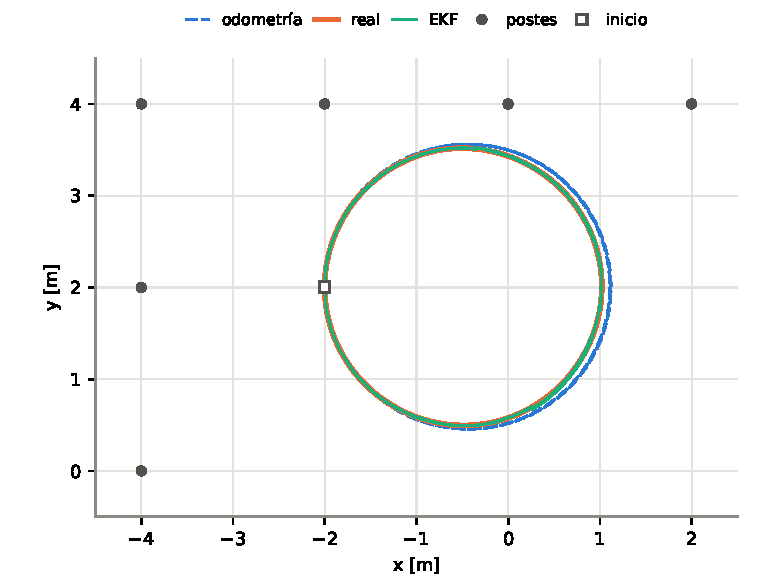
\includegraphics[width=\textwidth]{figuras/ekf_circulo_tray.pdf}
\caption{Trayectoria real y estimadas por la odometría y por el EKF, con velocidades constantes.}
\label{fig:ekf_circulo_tray}
\end{figure}

\begin{table}[htbp]
\centering
\begin{tabular}{lcc}
\toprule
\textbf{Error} & \textbf{EKF} & \textbf{Odometría} \\
\midrule
Posición medio [cm] & $1.2$ & $11.3$ \\
Posición máximo [cm] & $4.2$ & $22.4$ \\
Posición final [cm] & $0.4$ & $21.2$ \\
Orientación final & $0.1^\circ$ & $6.1^\circ$ \\
\bottomrule
\end{tabular}
\caption{Errores de la pose estimada por el EKF y por la odometría, con velocidades constantes.}
\label{tab:ekf_circulo}
\end{table}

La trayectoria estimada por el EKF se mantiene sobre la real durante todo el recorrido, mientras que la de la odometría se va separando de ella (Figura~\ref{fig:ekf_circulo_tray}). En la Figura~\ref{fig:ekf_circulo_error} y en la Tabla~\ref{tab:ekf_circulo} se ve que el error de la odometría crece con el tiempo, hasta llegar a $21$~cm y $6.1^\circ$ al final, mientras que el del EKF se mantiene en el orden de $1$~cm, ya que cada vez que el láser detecta postes la estimación se corrige.

\begin{figure}[htbp]
\centering
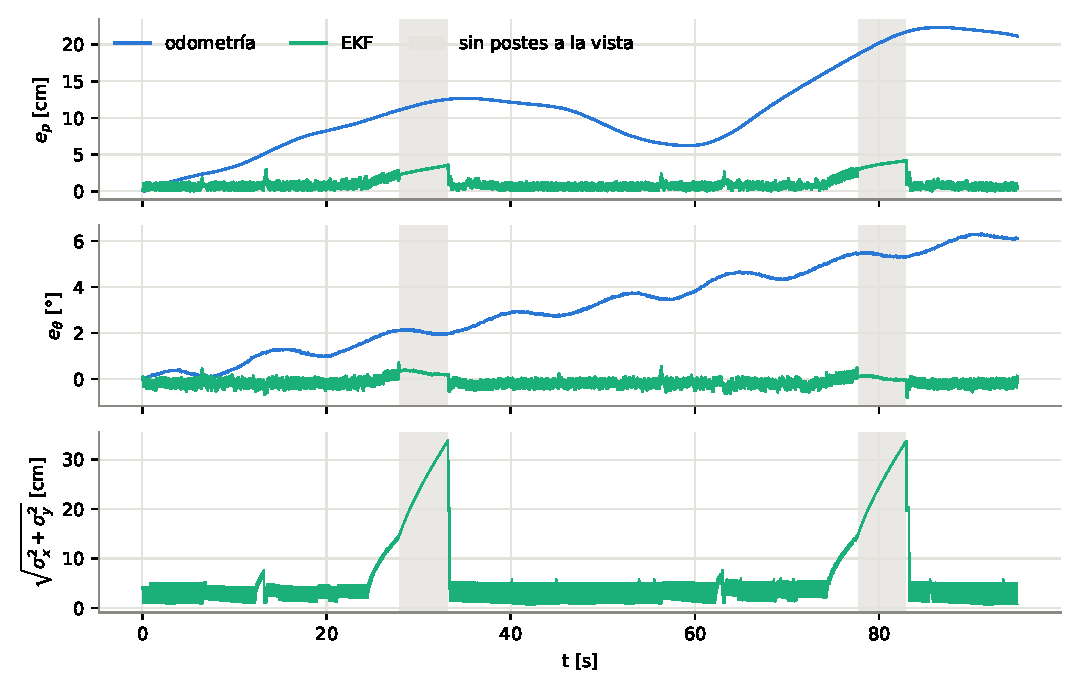
\includegraphics[width=\textwidth]{figuras/ekf_circulo_error.pdf}
\caption{Errores de posición y de orientación de la odometría y del EKF, y desvío de la posición que estima el EKF.}
\label{fig:ekf_circulo_error}
\end{figure}

La única excepción son dos tramos de unos $5$~s, uno en cada vuelta, en los que el láser no ve ningún poste. En ellos el filtro solo predice, de manera que su error crece igual que el de la odometría, hasta unos $4$~cm, y la incertidumbre que estima crece todavía más, hasta $34$~cm, porque $Q$ se suma en cada paso. Cuando el láser vuelve a ver postes la estimación se corrige, y tanto el error como la incertidumbre bajan de golpe. Esto muestra que lo que mejora la estimación no es el filtro por sí mismo, sino las observaciones de los postes.

Con postes a la vista, la incertidumbre oscila entre $1$ y $5$~cm, ya que crece con cada predicción y baja con cada corrección. Además, en más del $99\%$ de las muestras el error real del EKF se mantuvo por debajo de dos veces el desvío que estima el filtro, en las tres componentes de la pose, es decir, la incertidumbre que informa el filtro es mayor que su error real. Esto es lo que se espera al elegir $Q$ mayor que el error de la odometría en un paso.

En la Figura~\ref{fig:ekf_circulo_rviz} se muestra la elipse de covarianza de la posición en RViz2 a lo largo del recorrido, ampliada diez veces para que sea visible. Las elipses más grandes corresponden al tramo en el que el láser no ve postes.

Además, la forma de la elipse depende de cuántos postes ve el láser. Cuando ve uno solo, el rango medido fija con precisión la distancia al poste, pero no la posición en la dirección perpendicular, por lo que la elipse se alarga en esa dirección. Cuando no ve ninguno, la incertidumbre crece en todas las direcciones, y la elipse se agranda sin alargarse.

\begin{figure}[htbp]
\centering
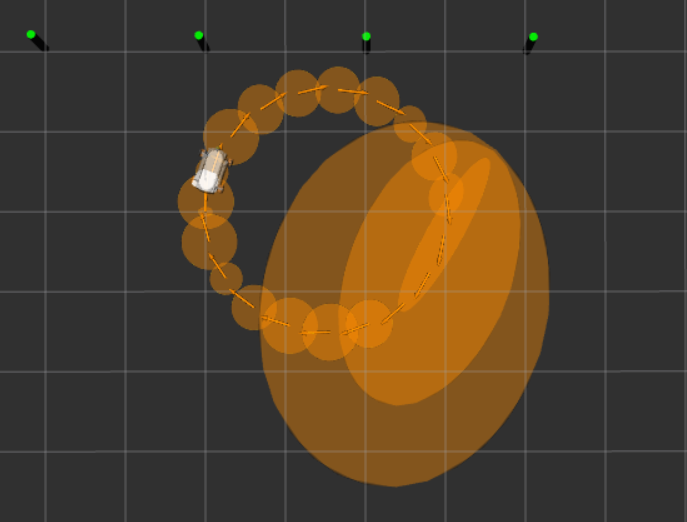
\includegraphics[width=0.45\textwidth]{figuras/ekf_circulo_rviz.png}
\caption{Elipse de covarianza del EKF en RViz2 durante la circunferencia, ampliada diez veces. Los puntos verdes son los postes que detecta el láser en ese instante.}
\label{fig:ekf_circulo_rviz}
\end{figure}

% =====================================================================
\section{Seguimiento de trayectorias a lazo cerrado utilizando localización basada en EKF}
Para seguir la trayectoria utilizando la estimación del EKF no fue necesario modificar el controlador. Como el controlador obtiene la pose del robot de la transformación \texttt{map} $\rightarrow$ \texttt{base\_frame}, alcanza con cambiar el parámetro \texttt{base\_frame} de \texttt{base\_link} a \texttt{base\_link\_ekf}, de manera que la retroalimentación pasa a ser la pose que publica el EKF. Se utilizaron las constantes elegidas en la Sección~\ref{sec:lazo_exp}, y no fue necesario volver a ajustarlas.

Para evaluar el sistema completo, se comparó una corrida con el EKF en el lazo con otra en la que el lazo se cierra con la odometría. En esta última, el EKF también estima la pose, pero el controlador no la utiliza. Las dos corridas siguen la misma trayectoria con las mismas constantes, por lo que la única diferencia es la pose que recibe el controlador.

\begin{figure}[htbp]
\centering
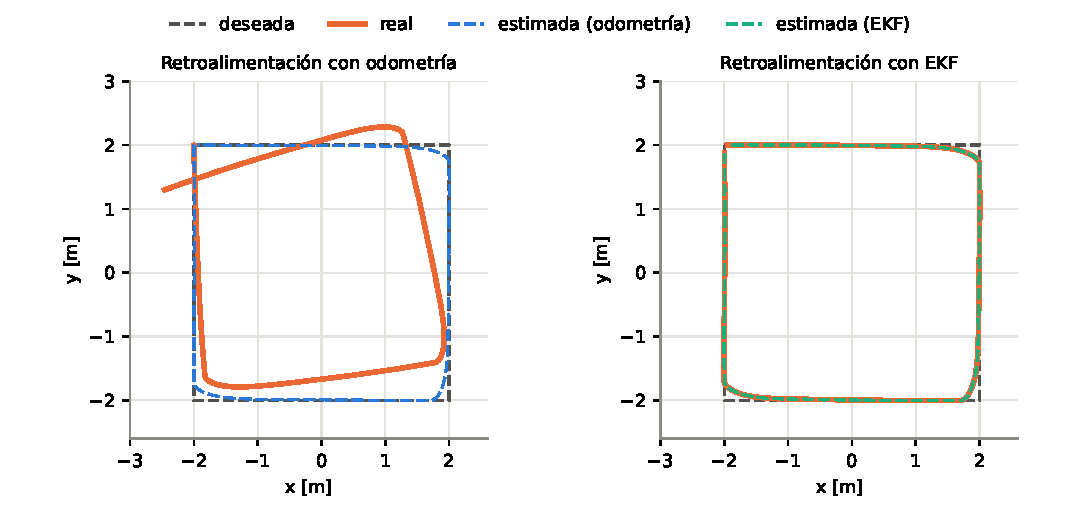
\includegraphics[width=\textwidth]{figuras/ekf_cuadrado_tray.pdf}
\caption{Trayectoria deseada, estimada y real, con la odometría y con el EKF como retroalimentación.}
\label{fig:ekf_cuadrado_tray}
\end{figure}

\begin{table}[!h]
\centering
\begin{tabular}{lcc}
\toprule
\textbf{Robot real} & \textbf{Con EKF} & \textbf{Con odometría} \\
\midrule
Distancia al cuadrado, media [cm] & $1.6$ & $21.5$ \\
Distancia al cuadrado, máxima [cm] & $14.3$ & $54.1$ \\
Error de orientación, medio & $0.5^\circ$ & $4.2^\circ$ \\
Error de orientación, máximo & $3.4^\circ$ & $22.3^\circ$ \\
Error final de posición [cm] & $5.1$ & $83.8$ \\
Error final de orientación & $1.0^\circ$ & $18.1^\circ$ \\
\bottomrule
\end{tabular}
\caption{Errores del robot real respecto de la trayectoria deseada, según la pose que utiliza el controlador.}
\label{tab:ekf_cuadrado}
\end{table}

Con la odometría en el lazo, el robot real se aparta del cuadrado de la misma forma que en la Sección~\ref{sec:lazo_exp}, y termina a $84$~cm del punto de llegada (Figura~\ref{fig:ekf_cuadrado_tray}). En cambio, con el EKF el robot real sigue al cuadrado con una distancia media de $1.6$~cm, y termina a $5$~cm del punto de llegada con $1^\circ$ de error de orientación (Tabla~\ref{tab:ekf_cuadrado}).

\begin{figure}[htbp]
\centering
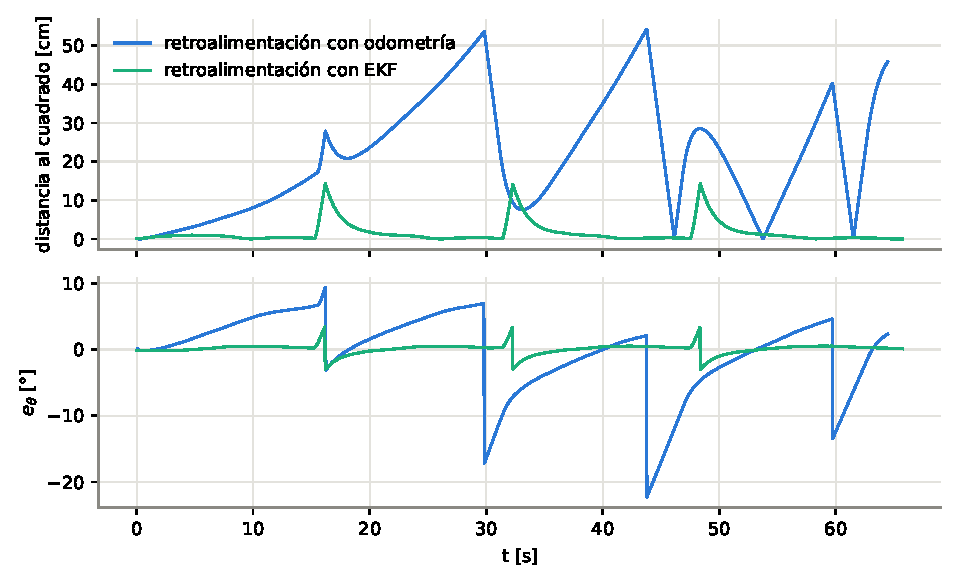
\includegraphics[width=\textwidth]{figuras/ekf_cuadrado_error.pdf}
\caption{Distancia del robot real al cuadrado y error de orientación respecto de la trayectoria, con la odometría y con el EKF como retroalimentación.}
\label{fig:ekf_cuadrado_error}
\end{figure}

Los picos de unos $14$~cm y $3^\circ$ que se ven en la Figura~\ref{fig:ekf_cuadrado_error} coinciden con los vértices, y no se deben a errores de localización, ya que el error del EKF respecto de la pose real se mantuvo por debajo de $2.3$~cm durante todo el recorrido. Se deben a que el robot recorta las esquinas por el \emph{lookahead}, al igual que en la Sección~\ref{sec:lazo_exp}.

Por último, en la Figura~\ref{fig:ekf_cuadrado_rviz} se muestra la elipse de covarianza en RViz2 a lo largo del recorrido, también ampliada diez veces. En el cuadrado el láser ve siempre entre $3$ y $5$ postes, por lo que la incertidumbre no crece como en la circunferencia, y las elipses tienen un tamaño parecido en los lados y en los vértices. Sus diferencias de tamaño se deben a que cada una se dibuja en un momento distinto del ciclo, en el que la incertidumbre crece con cada predicción y baja con cada corrección.

\begin{figure}[htbp]
\centering
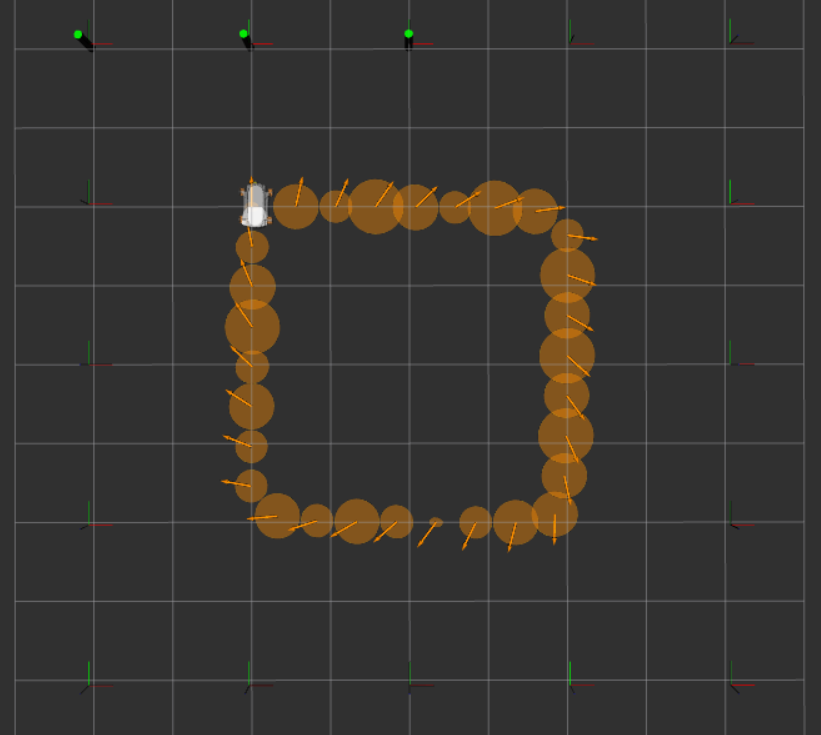
\includegraphics[width=0.45\textwidth]{figuras/ekf_cuadrado_rviz.png}
\caption{Elipse de covarianza del EKF en RViz2 durante el seguimiento del cuadrado, ampliada diez veces. Los puntos verdes son los postes que detecta el láser en ese instante.}
\label{fig:ekf_cuadrado_rviz}
\end{figure}

% =====================================================================
\section{Sistema desarrollado}
\subsection{Paquetes y nodos}

El sistema está compuesto por cinco paquetes de ROS2. Tres de ellos contienen los nodos (Tabla~\ref{tab:nodos}) y se corresponden con las tres etapas descriptas en la introducción. Los otros dos son de la materia y contienen lo que los nodos necesitan para funcionar, dado que \texttt{robmovil\_msgs} tiene los mensajes de los encoders, la trayectoria y los landmarks, y \texttt{kfilter} es la librería que contiene la clase \texttt{EKFilter}.

\begin{table}[htbp]
\centering
\small
\begin{tabular}{lll}
\toprule
\textbf{Paquete} & \textbf{Ejecutable} & \textbf{Función} \\
\midrule
\texttt{modelo\_holonomico} & \texttt{mecanum\_odometry\_node} & Cinemática inversa y odometría (Sección~\ref{sec:modelo}) \\
\texttt{lazo\_cerrado} & \texttt{trajectory\_generator} & Generación de la trayectoria (Sección~\ref{sec:trayectoria}) \\
 & \texttt{trajectory\_follower} & Controlador y \emph{pursuit} (Sección~\ref{sec:lazo_cerrado}) \\
\texttt{robmovil\_ekf} & \texttt{landmark\_detector\_node} & Detección de postes (Sección~\ref{sec:landmarks}) \\
 & \texttt{localizer} & Filtro EKF (Sección~\ref{sec:nodo_ekf}) \\
\bottomrule
\end{tabular}
\caption{Nodos implementados.}
\label{tab:nodos}
\end{table}

\subsection{Tópicos y transformaciones}

La comunicación de los nodos entre sí y con el simulador, cuando el robot sigue la trayectoria utilizando la estimación del EKF, se representa en la Figura~\ref{fig:sistema}. El controlador no recibe la pose por un tópico, sino que la obtiene de una transformación, de manera que para pasar de utilizar la odometría a utilizar el EKF alcanza con cambiar el parámetro \texttt{base\_frame} de \texttt{base\_link} a \texttt{base\_link\_ekf}.

\begin{figure}[htbp]
\centering
\begin{tikzpicture}[scale=0.85, transform shape, >=Stealth,
  blk/.style={draw, rectangle, minimum width=3.2cm, minimum height=1cm, align=center, font=\ttfamily\small},
  lab/.style={font=\ttfamily\scriptsize, align=center}]
  \node[blk, minimum height=5.2cm, minimum width=2.2cm, font=\small] (sim) at (0,0) {Simulador};
  \node[blk] (odo) at (6.7,2) {mecanum\_odometry};
  \node[blk] (det) at (6.7,-2) {landmark\_detector};
  \node[blk] (fol) at (13.3,2) {trajectory\_follower};
  \node[blk] (gen) at (13.3,4.2) {trajectory\_generator};
  \node[blk] (ekf) at (13.3,-2) {localizer};
  \draw[->] ($(odo.west)+(0,0.25)$) -- node[lab, above] {/robot/*\_wheel/cmd\_vel} ($(sim.east)+(0,2.25)$);
  \draw[->] ($(sim.east)+(0,1.75)$) -- node[lab, below] {/robot/encoders} ($(odo.west)+(0,-0.25)$);
  \draw[->] ($(sim.east)+(0,-2)$) -- node[lab, above] {/robot/front\_laser/scan} (det.west);
  \draw[->] (det.east) -- node[lab, above] {/landmarks} (ekf.west);
  \draw[->] (odo.south east) -- node[lab, right, pos=0.35, xshift=3pt] {/robot/odometry} (ekf.north west);
  \draw[->] (fol.west) -- node[lab, above] {/robot/cmd\_vel} (odo.east);
  \draw[->] (gen.south) -- node[lab, right] {/robot/trajectory} (fol.north);
  \draw[->, dashed] (ekf.north) -- node[lab, right] {map $\rightarrow$\\base\_link\_ekf} (fol.south);
  \draw[->] (sim.south) |- ++(1,-0.8) -| node[lab, above, pos=0.25] {/posts} (ekf.south);
\end{tikzpicture}
\caption{Nodos del sistema y tópicos que los conectan. La línea punteada indica una transformación.}
\label{fig:sistema}
\end{figure}

Los mensajes de cada tópico se detallan en la Tabla~\ref{tab:topicos}. Además de los que aparecen en la figura, se incluyen otros que ningún nodo necesita para funcionar, pero que sirven para visualizar el sistema en RViz2 o para registrar los experimentos.

\begin{table}[htbp]
\centering
\small
\begin{tabular}{lll}
\toprule
\textbf{Tópico} & \textbf{Mensaje} & \textbf{Publica} \\
\midrule
\texttt{/robot/encoders} & \texttt{robmovil\_msgs/MultiEncoderTicks} & Simulador \\
\texttt{/robot/front\_laser/scan} & \texttt{sensor\_msgs/LaserScan} & Simulador \\
\texttt{/posts} & \texttt{geometry\_msgs/PoseArray} & Simulador \\
\texttt{/robot/*\_wheel/cmd\_vel} & \texttt{std\_msgs/Float64} & \texttt{mecanum\_odometry} \\
\texttt{/robot/odometry} & \texttt{nav\_msgs/Odometry} & \texttt{mecanum\_odometry} \\
\texttt{/robot/trajectory} & \texttt{robmovil\_msgs/Trajectory} & \texttt{trajectory\_generator} \\
\texttt{/robot/cmd\_vel} & \texttt{geometry\_msgs/Twist} & \texttt{trajectory\_follower} \\
\texttt{/landmarks} & \texttt{robmovil\_msgs/LandmarkArray} & \texttt{landmark\_detector} \\
\midrule
\texttt{/desired\_path} & \texttt{nav\_msgs/Path} & \texttt{trajectory\_generator} \\
\texttt{/goal\_pose} & \texttt{geometry\_msgs/PoseStamped} & \texttt{trajectory\_follower} \\
\texttt{/real\_path} & \texttt{nav\_msgs/Path} & \texttt{trajectory\_follower} \\
\texttt{/robot/odometry\_ekf} & \texttt{nav\_msgs/Odometry} & \texttt{localizer} \\
\texttt{/landmark\_markers} & \texttt{visualization\_msgs/MarkerArray} & \texttt{landmark\_detector} \\
\bottomrule
\end{tabular}
\caption{Tópicos del sistema. Los últimos cinco se utilizan para visualización y registro.}
\label{tab:topicos}
\end{table}

A su vez, las poses se comparten a través de las transformaciones de la Tabla~\ref{tab:tf}. La pose real, \texttt{base\_link\_gt}, no es entrada de ningún nodo, sino que solo se utiliza para evaluar los resultados.

\begin{table}[htbp]
\centering
\small
\begin{tabular}{lll}
\toprule
\textbf{Transformación} & \textbf{Publica} & \textbf{Contenido} \\
\midrule
\texttt{map} $\rightarrow$ \texttt{odom} & Simulador & Pose inicial del robot en el mapa \\
\texttt{odom} $\rightarrow$ \texttt{base\_link\_gt} & Simulador & Pose real \\
\texttt{base\_link} $\rightarrow$ \texttt{front\_laser} & Simulador & Posición del láser en el robot \\
\texttt{odom} $\rightarrow$ \texttt{base\_link} & \texttt{mecanum\_odometry} & Pose estimada por odometría \\
\texttt{map} $\rightarrow$ \texttt{base\_link\_ekf} & \texttt{localizer} & Pose estimada por el EKF \\
\bottomrule
\end{tabular}
\caption{Transformaciones del sistema.}
\label{tab:tf}
\end{table}

\subsection{Instrucciones de ejecución}

El sistema se ejecuta dentro del contenedor de Docker de la materia, que incluye ROS2 Humble y CoppeliaSim. En el archivo \texttt{start-docker.sh}, de la carpeta \texttt{ros\_docker}, está escrita la ruta del repositorio en la computadora, por lo que se debe modificar según dónde se lo haya clonado. Luego, desde esa carpeta, se crea la imagen, se inicia el contenedor y se abre una terminal dentro de él.

\begin{verbatim}
bash start-docker.sh build
bash start-docker.sh start
bash start-docker.sh open
\end{verbatim}

Para que el simulador publique los encoders y los postes, los mensajes \texttt{MultiEncoderTicks} y \texttt{PoseArray} deben estar declarados en el paquete \texttt{sim\_ros2\_interface}, como se indica en el anexo de la consigna. Luego se compila el workspace.

\begin{verbatim}
cd /root/ros2_ws
colcon build --symlink-install
source install/setup.bash
\end{verbatim}

Con el workspace compilado, se abre CoppeliaSim con el comando \texttt{coppeliaSim.sh} y se carga la escena \texttt{coppeliaSim/omni\_ekf.ttt}. Como el simulador publica los postes una sola vez, al iniciar la simulación, los nodos tienen que estar corriendo antes. Por eso, primero se ejecuta el sistema completo en otra terminal del contenedor, y luego se inicia la simulación para que el robot siga la trayectoria utilizando la estimación del EKF.

\begin{verbatim}
ros2 launch robmovil_ekf seguimiento_ekf.launch.py
\end{verbatim}

Si en cambio se quiere seguir la trayectoria utilizando solo la odometría, se ejecuta el siguiente comando, en el que también se pueden elegir las constantes del controlador.

\begin{verbatim}
ros2 launch lazo_cerrado seguimiento_odom.launch.py kp_xy:=0.8 kp_yaw:=0.75
\end{verbatim}

Por último, para mover el robot con velocidades constantes y sin el controlador, se ejecutan la odometría y el EKF, se inicia la simulación y se publica la velocidad deseada, cada comando en una terminal distinta.

\begin{verbatim}
ros2 launch modelo_holonomico odometry.launch.py
ros2 launch robmovil_ekf localizer.launch.py
ros2 topic pub -r 10 /robot/cmd_vel geometry_msgs/msg/Twist \
  "{linear: {x: 0.1, y: 0.0}, angular: {z: 0.1}}"
\end{verbatim}

En todos los casos, el sistema se puede visualizar en RViz2 con la configuración \texttt{tpfinal.rviz} de la carpeta \texttt{coppeliaSim}, que utiliza el modelo del robot \texttt{URDF/holonomico.urdf}.

% =====================================================================
\section{Conclusiones}

En este trabajo se implementó un sistema que permite a un robot omnidireccional de cuatro ruedas Mecanum seguir una trayectoria cuadrada, combinando el modelo cinemático de la plataforma, un controlador proporcional y un EKF que corrige la estimación de la pose a partir de los postes del entorno.

El modelo cinemático permite comandar al robot en las tres direcciones de manera independiente, y la odometría reproduce la forma de las trayectorias, pero acumula un error que no tiene forma de detectar, ya que las ruedas deslizan y los encoders solo miden cuánto giran. Este error es mayor cuanto más rápido se mueve el robot y en el desplazamiento lateral, y en el recorrido del cuadrado, de unos $16$~m, llega a casi $1$~m.

Con el controlador ocurre algo similar, dado que sigue correctamente a la pose estimada con cualquiera de las constantes probadas, pero como se retroalimenta con la odometría, el robot real se aparta del cuadrado. Las constantes elegidas, $k_{p,xy} = 0.8$ y $k_{p,yaw} = 0.75$, mantienen una velocidad moderada y orientan al robot según la trayectoria en el lugar en el que se encuentra, pero no pueden corregir el error de la odometría.

El EKF resuelve este problema, ya que corrige la estimación cada vez que el láser detecta postes. Con velocidades constantes, el error de la pose estimada bajó de $11$~cm con la odometría a $1$~cm con el EKF, y al utilizarlo como retroalimentación, el robot real siguió al cuadrado con una distancia media de $1.6$~cm, contra $21.5$~cm con la odometría, y terminó a $5$~cm del punto de llegada, contra $84$~cm. A su vez, se vio que la mejora depende de las observaciones, de manera que en los tramos en los que el láser no ve postes el filtro solo predice y la incertidumbre crece.

El principal problema que se encontró es el deslizamiento de las ruedas, que la odometría no puede medir y el controlador no puede corregir por sí solo. Si bien el EKF lo resuelve mientras el láser ve postes, en los tramos en los que no ve ninguno la estimación vuelve a depender de la odometría y su error crece, por lo que una posible mejora sería agregar más postes en el recorrido, o un sensor que permita medir el giro del robot sin depender de las ruedas. A su vez, el robot recorta las esquinas del cuadrado hasta $14$~cm, por anticipar el objetivo, lo que se podría reducir disminuyendo el \emph{lookahead} cerca de los vértices. Por último, de cada configuración del controlador se realizó una sola corrida, por lo que repetirlas permitiría confirmar que las diferencias entre las constantes no se deben a la variabilidad entre corridas.

De esta forma, se logró que el robot siga la trayectoria de referencia de manera precisa, como se propuso al comienzo del trabajo, y se vio que para lograrlo no alcanza con un buen controlador, sino que también es necesario contar con una buena estimación de la pose.

% =====================================================================
\appendix
\begin{thebibliography}{9}
\bibitem{taheri2015} H.~Taheri, B.~Qiao y N.~Ghaeminezhad. \emph{Kinematic Model of a Four Mecanum Wheeled Mobile Robot}. International Journal of Computer Applications, 113(3), 2015.
\bibitem{consigna} \emph{TP Final: Seguimiento de trayectoria a lazo cerrado basado en EKF para un robot omnidireccional}. Robótica Móvil, FCEyN, UBA, 2do cuatrimestre 2025.
\end{thebibliography}

\section{Anexo: parámetros utilizados}

En la Tabla~\ref{tab:anexo} se resumen los parámetros utilizados por cada nodo, con los valores con los que se realizaron los experimentos.

\begin{table}[!htbp]
\centering
\small
\begin{tabular}{lll}
\toprule
\textbf{Nodo} & \textbf{Parámetro} & \textbf{Valor} \\
\midrule
\texttt{mecanum\_odometry} & Radio de rueda $r$ & $0.05$~m \\
 & Semidistancia entre ruedas $(l_x + l_y)/2$ & $0.175$~m \\
 & Resolución del encoder & $500$ ticks/rev \\
\midrule
\texttt{trajectory\_generator} & Semilado del cuadrado & $2$~m \\
 & Separación entre waypoints & $0.05$~m \\
\midrule
\texttt{trajectory\_follower} & $k_{p,xy}$ & $0.8$ \\
 & $k_{p,yaw}$ & $0.75$ \\
 & \emph{Lookahead} & $0.30$~m \\
 & Tolerancia de posición al final & $0.05$~m \\
 & Tolerancia de orientación al final & $0.05$~rad \\
 & Frecuencia de control & $30$~Hz \\
\midrule
\texttt{landmark\_detector} & Distancia máxima entre puntos de un grupo & $0.15$~m \\
 & Puntos por grupo & entre $2$ y $30$ \\
 & Rango máximo & $8$~m \\
 & Diámetro de los postes & $0.1$~m \\
\midrule
\texttt{localizer} & $\sigma_x$, $\sigma_y$ (por paso) & $0.02$~m \\
 & $\sigma_\theta$ (por paso) & $0.01$~rad \\
 & $\sigma_r$ & $0.01$~m \\
 & $\sigma_\varphi$ & $0.005$~rad \\
 & $P_0$ & $0.01 \cdot I_3$ \\
 & Distancia máxima de asociación & $0.6$~m \\
 & Rango mínimo de una observación & $0.2$~m \\
\bottomrule
\end{tabular}
\caption{Parámetros utilizados en cada nodo.}
\label{tab:anexo}
\end{table}

\end{document}
